%problem 1
\section{Problem 1, Symbol Tables}
\subsubsection{What is a symbol table, and why is it needed?}
A symbol table is a data structure used by compilers and interpreters that holds the identifiers and relevant information found in the source code of the program.
Such as where a symbol is used.

Variable and function and class names and such are very useful for programmers to tell stuff apart in the code and can also carry some semantic value that aids the programmer in figuring out what the code does.
However computers don't care what a variable is called, as long as it doesn't confuse it with another variable.
Once the symbol table is complete, the identifiers can be replaced with more machine friendly values (e.g. references to an entry in the symbol table).
The symbol table is used in the process of translating variable and function names to addresses and offsets and what not.
You know, whatever the architecture we are compiling for uses.

Also it's useful during error checking.
Type checking (did we try and assign a string to an integer variable?), declaration checking (or whatever, that we don't try and declare more than one thing with the same identifier within the same scope or whatever the language's rules are -- name collisions?).

Strictly speaking, it is not needed.
Instead of looking something up in the symbol table we could search through the code.
Though this is computationally expensive compared to using a hash table to store what we've already found.
So in the sense that it is computationally wasteful to \emph{not} have a symbol table, I suppose you could say it is needed.


\subsubsection{What kind of information is typically stored in a symbol table?}
Well you know, stuff.
Like what's listed below or in section 8.3.3 of the handout for this assignment.
\begin{description}
	\item[Name] the symbol's identifier
	\item[Type] the symbol's type
	\item[Scope] the scope the symbol was declared in
	\item[References] references to the symbol found in the code
\end{description}

\subsubsection{Mention and briefly discuss the advantages and disadvantages of three different data structures that can be used to implement symbol tables.}
\paragraph{Linked list}

You know, just a regular linked list or an array or whatever.
The kind where each entry points to the next one and we have to scan the entries sequentially when searching.

Advantages: Easy to implement, O(1) insertion\\
Disadvantages: O(n) lookup, 


\paragraph{Hash table}

Using the identifier as the key.

Advantages: O(1) everything\\
Disadvantages: people might think you're talking about drugs

\paragraph{Binary search tree}

Using the identifier as the key.
This would allow us to find almost matching identifiers when searching through the tree.
However we are typically only interested in knowing if a value is already in the symbol table already or not.
Also it'd probably be a good idea to use a self-balancing tree.

Advantages: O(log n) everything, not very difficult to implement\\
Disadvantages: only O(log n) everything if it's balanced.

\newpage
\setcounter{subsubsection}{0}
% problem 2
\section{Problem 2, Symbol tables and blocks}
Consider the following code in a version of [VSL] that includes the keyword \texttt{BLOCK} to start a new scope:
\begin{figure}[H]
\begin{verbatim}
VOID FUNC main() START
    int a;
    FLOAT b;
    ...
    BLOCK
        bool b;
        ... // Position 1
    END

    BLOCK
        int b;
        FLOAT c;
        ...
        BLOCK
            BOOL a;
            INT c;
            ... // Position 2
        END
    END
END
\end{verbatim}
\end{figure}

\subsubsection{Show the contents of the symbol tables at position 1 and 2 assuming an implementation using a stack of symbol tables.}
% so with the stack of symbol tables we'd have one ST per scope?
So, we create a new symbol table as we enter a block/scope and stop adding stuff to it when we leave the block/scope?
Is this the same thing as chained symbol tables (Fig 2.36, pg 88 of \textsc{drag on book})?
Because that is what I am betting on.

\begin{figure}[H]
\Tree [.Global\\main:function;void [.main\\a:int\\b:float [.main-0\\b:bool ]  ] ]
\label{fig:2-a-1}
\caption{The contents of the symbol table at position 1, using a stack of symbol tables. Shown as a tree.}
\end{figure}
%TODO: make a proper tree with tables or whatever. Like in Fig 2.36@pg88. So learn TikZ? Yeah ok.

\begin{figure}[H]
\Tree [.Global\\main:function;void [.main\\a:int\\b:float [.main-0\\b:bool ] [.main-1\\b:int\\c:float [main-1-0\\a:bool\\c:int ] ] ] ]
\label{fig:2-a-2}
\caption{The contents of the symbol table at position 2, using a stack of symbol tables. Shown as a tree.}
\end{figure}
%TODO: join these! Make them one! (use subfigures like in the last theory assignment)

\subsubsection{Show the contents of the symbol tables at position 1 and 2 assuming an implementation using a single symbol table.}
I can just make up the scope names as I go along, right?
I mean what the scopes are called shouldn't matter as long as I get the identifiers right, right?

Also what is ``a single symbol table''supposed to mean?
Is the point that we can't have scopes with just a single symbol table?
I don't know, man. 
I can't remember either of these two approaches being mentioned in any of the lectures, and I couldn't find anything about them in the slides.
The book seems to use the stack-based approach, in the sense that a new symbol table is created for each scope.
If a new symbol table is not created for each scope, we'd just be putting all the names in the same symbol table.
However the type of symbol table we choose to use shouldn't affect the language.
So scopes and such should still work, which means we do have to reset the offset and list each name's scope along with its entry in the table.

I don't think I get it.

Oh, wait, nevermind.
It's in the handout!
The answers, they were all in the handout all along!

\begin{table}[H]
\begin{subtable}[h]{0.5\textwidth}
	\hfill
	\begin{tabular}{|c|l|l|}
		\hline
		Identifier & Type			& Scope \\ \hline
		main	& function, void& global \\
		a		& int			& main	\\
		b		& float			& main	\\
		b		& bool			& main-0 \\
		\hline
	\end{tabular}
	\label{tab:2-b-1}
	\caption{The contents of the symbol table at position 1, using a single symbol table.}
\end{subtable}
\begin{subtable}[h]{0.5\textwidth}
	\hfill
	\begin{tabular}{|c|l|l|}
		\hline
		Identifier& Type			& Scope \\ \hline
		main	& function, void& global \\
		a		& int			& main	\\
		b		& float			& main	\\
		b		& bool			& main-0 \\
		b		& int			& main-1 \\
		c		& float			& main-1 \\
		a		& bool			& main-1-0 \\
		c		& int			& main-1-0 \\
		\hline
	\end{tabular}
	\label{tab:2-b-2}
	\caption{The contents of the symbol table at position 2, using a single symbol table.}
\end{subtable}
	\label{tab:2-b}
	\caption{The contents of the symbol table.}
\end{table}

\subsubsection{What are the advantages and disadvantages of these approaches?}
Both approaches contain the same information.
I think the stack one looks nicer.
It makes for better illustrations because it better illustrates which scopes are under which.

Is it something about their implementations and how the stack one is segmented rather than just one huge table?
Yeah, that's it.
With the stack-based approach we might have to search more than one symbol table to find what we are looking for.
But we would never have to search through all of them because we are only interested in entries in scopes located above the one we are in.

Also you could implement the stack approach as a two-tiered hash table (scope as the outside key, identifier as the inside key) and have pointers or references or whatever to the parent scope of a scope.
Worst case would be if there are no adjacent scopes and we have to look through all of them, which is still just $O(n)$ in worst case ($n$ is the number of symbol tables).
Worst case for the single table would be that we have to look through all of it manually ($O(m)$ ($m$ is the number of symbols in the table)) but I can't think of a situation like that.

If the scope tree for a ``typical'' program written in the language we are working with tends to be balanced, then the stack approach is nice.

Also see what I wrote on a) and b) because there are some words there that are relevant to this question as well.
Man, \emph{words}.

\newpage
\setcounter{subsubsection}{0}
% problem 3
\section{Problem 3, Type checking}
\subsubsection{What is the difference between type synthesis and type inference?}
Type synthesis and type inference are both forms of type checking\footnote{Type checking is when you check that the type expressions you found in a source program conform to the source language's type system.}.

\emph{Type synthesis} builds/figures out the type of an expression by looking at its subexpressions.
For example, the type of the name \emph{z} in the expression \texttt{z = x+y} would be whatever the language's type system says that the type of \emph{x} added to the type of \emph{y} should be.
If \emph{x} and \emph{y} are integers in a language that has no other types than integers, the type of \emph{z} would probably be an integer.
It's hard to say for sure if we don't know what the language's type system is like.
Type synthesis requires that names are declared before use.

\emph{Type inference} determines the type of a name from the way it is used.
For example, if \emph{x} is used as an argument to a function that specifies that its parameter should have type \emph{t} then the type of \emph{x} must be \emph{t}.
Actually the type of \emph{x} could be anything, but if it's not \emph{t} then we'll get an error.

\subsubsection{Some languages, e.g. FORTRAN, have native support for complex numbers. Draw the widening conversions/hierarchy for the following set of types: \texttt{int}, \texttt{float}, \texttt{double}, \texttt{complex int}, \texttt{complex float}, \texttt{complex double}. State the assumptions you make.}
%Check out Fig 6.25 on pg 389 for an example of widening conversion.
%Casting can be done upwards in the tree without loss of information.
\begin{figure}[H]
Assumptions: 
\begin{itemize}
	\item The width of \emph{complex t} is twice the width of \emph{t} 
	\item Names of type \emph{t} can be converted to \emph{complex t} without loss of information by copying the real part and letting the imaginary part be zero.
	\item Conversions can be done upwards in the tree without loss of information (see \textsc{DB} page 388).
\end{itemize}
\end{figure}

\begin{figure}[H]
% oh right there's supposed to be a tree here
%TODO: make the tree here
% it's just c double > c float > c int
% 			double	 >	 float >   int
\centering
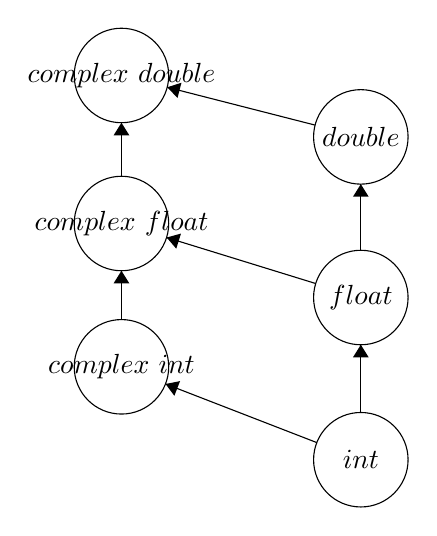
\begin{tikzpicture}[scale=0.2]
\tikzstyle{every node}+=[inner sep=0pt]
\draw [black] (19.4,-21.5) circle (3);
\draw (19.4,-21.5) node {$complex\mbox{ }double$};
\draw [black] (19.4,-30.9) circle (3);
\draw (19.4,-30.9) node {$complex\mbox{ }float$};
\draw [black] (19.4,-40) circle (3);
\draw (19.4,-40) node {$complex\mbox{ }int$};
\draw [black] (34.6,-25.4) circle (3);
\draw (34.6,-25.4) node {$double$};
\draw [black] (34.6,-35.6) circle (3);
\draw (34.6,-35.6) node {$float$};
\draw [black] (34.6,-45.9) circle (3);
\draw (34.6,-45.9) node {$int$};
\draw [black] (19.4,-27.9) -- (19.4,-24.5);
\fill [black] (19.4,-24.5) -- (18.9,-25.3) -- (19.9,-25.3);
\draw [black] (19.4,-37) -- (19.4,-33.9);
\fill [black] (19.4,-33.9) -- (18.9,-34.7) -- (19.9,-34.7);
\draw [black] (31.8,-44.81) -- (22.2,-41.09);
\fill [black] (22.2,-41.09) -- (22.76,-41.84) -- (23.12,-40.91);
\draw [black] (34.6,-42.9) -- (34.6,-38.6);
\fill [black] (34.6,-38.6) -- (34.1,-39.4) -- (35.1,-39.4);
\draw [black] (31.73,-34.71) -- (22.27,-31.79);
\fill [black] (22.27,-31.79) -- (22.88,-32.5) -- (23.18,-31.54);
\draw [black] (34.6,-32.6) -- (34.6,-28.4);
\fill [black] (34.6,-28.4) -- (34.1,-29.2) -- (35.1,-29.2);
\draw [black] (31.69,-24.65) -- (22.31,-22.25);
\fill [black] (22.31,-22.25) -- (22.96,-22.93) -- (23.21,-21.96);
\end{tikzpicture}

\caption{The widening conversions for the set of types presented in the problem text.}
\label{fig:3-b}
\end{figure}

\newpage
\setcounter{subsubsection}{0}
% problem 4
\section{Problem 4, Types, SDDs}
Consider the following partially completed SDD for type expressions:
\begin{table}[H]
\begin{tabular}{ll}
	\textsc{Production} & \textsc{Semantic Rule} \\ \hline
	T ::= \textbf{int}	&						\\
	T ::= \textbf{float}& \\
	T ::= \textbf{bool} & \\
	T ::= \textbf{T[num]}& \\
	T ::= (L) 			& \\
	L ::= L,T			& \\
	L ::= T				& \\
\end{tabular}
\end{table}

Possible types are the basic types \textbf{int}, \textbf{float}, and \textbf{bool}, arrays of any kind of type, e.g. \textbf{int}[5] or \textbf{float}[5][4] and records (which are collections of one or more types, e.g. \textbf{int}, \textbf{float}, (\textbf{int, bool}[3])).

The purpose of the SDD is to compute the number of bytes that must be allocated to store a value of a given type.
\begin{itemize}
	\item \textbf{int} requires 4 bytes, \textbf{float} requires 8 bytes, \textbf{bool} requires 1 byte.
	\item An array requires the number of bytes a single element, multiplied by the length of the array. For instance, \textbf{int}[5] would require 20 bytes. Similarily, \textbf{int}[5][5] (where the type of the elements is \textbf{int}[5]) would require 100 bytes.
	\item A record requires the sum of bytes required by its members. That is, (\textbf{int, bool}[5]) would require 9 bytes.
\end{itemize}

\subsubsection{Complete the SDD, so that the \textit{size} attribute of T stores the size of the type.}
%p304
% SDD = Syntax Directed Definition
I changed the fourth production to $T\rightarrow T_{1}[\mathbf{num}]$ because that's the kind of notation used in the book.
It also eliminates the possibility that the rule be misunderstood as $x=x$ or some other tautology.
A similar change was made to the sixth production.
\begin{table}[H]
\centering
\begin{tabular}{l|l}
	\hline \hline
	\textsc{Production} 			& \textsc{Semantic Rule} \\ \hline
	$T \rightarrow \mathbf{int}$			& $T.size = 4$	\\
	$T \rightarrow \mathbf{float}$			& $T.size = 8$	\\
	$T \rightarrow \mathbf{bool}$ 			& $T.size = 1$	\\
	$T \rightarrow T_{1}\mathbf{[num]}$		& $T.size = T_1.size * \mathbf{num}.lexval$\\
	$T \rightarrow (L)$ 					& $T.size = L.size$ \\
	$L \rightarrow L_{1},T$					& $L.size = L_1.size + T.size$	\\
	$L \rightarrow T$						& $L.size = T.size$	\\
	\hline
\end{tabular}
\label{tab:4-a}
\caption{The completed SDD.}
\end{table}

\subsubsection{Show annotated parse trees for each of these types:}
\begin{description}
	\item[i)] \textbf{int}[4][3][5] \\
		See Figure~\ref{fig:4-b-i}.
	\item[ii)] (\textbf{int}, \textbf{float}, (\textbf{bool}, \textbf{int}[4])) \\
		See Figure~\ref{fig:4-b-ii}.
\end{description}

All right, done in the style found in Figure 5.3 and 5.5 on page 308-9 of the \textsc{D???} book.
%TODO: make this a figure.
%TODO: make another one for the other thing
\begin{figure}[H]
\Tree [.{$T.size = 240$} 
		[.{$T.size = 48$} 
			[.{$T.size = 16$}
				[.{$T.size = 4$} {$\mathbf{int}.size = 4$} ]
			{[} {$\mathbf{num}.lexval = 3$} {]} ]
		!\qsetw{1cm} {[} {$\mathbf{num}.lexval = 4$} {]} ] 
	  !\qsetw{1cm} {[} {$\mathbf{num}.lexval = 5$} {]} ] 
% !\qsetw{1cm} sets the width of the subtree to 1cm
% I tried placing it on the first line just after the } of the root node, but that didn't work

\caption{Annotated parse tree for ``\textbf{int}[4][3][5]''.}
\label{fig:4-b-i}
\end{figure}


\begin{figure}[H]
\Tree	[.{$T.size = 29$} {(} %a
			[.{$L.size = 29$} %b
				[.{$L.size = 12$} %c
					[.{$L.size = 4$} [.{$T.size = 4$} {$\mathbf{int}.size = 4$} ] % d, e
					]
				{,}
					[.{$T.size = 8$}
						[{$\mathbf{float}.size = 8$} ]
					] %f
				]
			{,}
				[.{$T.size = 17$}  % g
				{(}
					[.{$L.size = 17$} % h
						[.{$L.size = 1$}  %i
							[.{$T.size = 1$} {$\mathbf{bool}.size = 1$} %j
							]
						]
					{,}
						[.{$T.size = 16$} %k
							[.{$T.size = 4$} {$\mathbf{int}.size = 4$} ] %l
						%!\qsetw{2.5cm}
						{[}
						{$\mathbf{num}.lexval = 4$}
						!\qsetw{2.5cm} %affects children of k
						{]}
						] !\qsetw{4.5cm} %affects children of h
					 ] !\qsetw{2.5cm} %affects children of g %
				 {)}
				]  !\qsetw{2.5cm} % affects children of c
			] !\qsetw{2.5cm} % affects children of a/the root
		 {)}
		 ]

\caption{Annotated parse tree for ``(\textbf{int}, \textbf{float}, (\textbf{bool}, \textbf{int}[4]))''.}
\label{fig:4-b-ii}
\end{figure}

% problem 5
\newpage
\section{Problem 5, SDDs}
????
